\documentclass[brazilian, 8pt, a4paper, final]{article}
\usepackage[utf8]{inputenc}
\usepackage[brazil]{babel}
\usepackage[T1]{fontenc}
\usepackage{multicol}
\usepackage{graphicx}
\usepackage{indentfirst}
\usepackage{float}
\usepackage{amsmath}
\usepackage{array}
\usepackage{caption}
\usepackage[left=1.5cm, right=1.5cm]{geometry}

\title{\textbf{Movimento de Foguetes}}

\author{Cristiane de Paula Oliveira\\\\\small{Instituto de Física -- Universidade Federal do Rio Grande do Sul}}

\begin{document}

\maketitle

\begin{abstract}
  \noindent
  Neste trabalho buscou-se estudar o movimento de foguetes. Para isso, foram desenvolvidos modelos matemáticos baseados na análise do {\em momentum} linear do foguete. No primeiro momento, estuda-se o movimento de foguetes no espaço livre. Depois, considera-se o movimento de ascensão vertical sob ação da gravidade. Por último, leva-se em conta também a resistência do ar na ascensão vertical sob gravidade. Este último problema não possui solução analítica. Utilizaram-se os métodos de Euler, de Runge-Kutta de $2^{a}$ e $4^{a}$ ordem para encontrar soluções numéricas de cada problema.
  \\ \textbf{Palavras-chave:} movimento de foguetes; solução numérica; método de Euler; método de Runge-Kutta
\end{abstract}


\begin{multicols*}{2}
\section{Introdução}
Um problema interessante para a aplicação da dinâmica de Newton é o movimento de foguetes simplificados. Métodos numéricos podem ser particularmente úteis para resolução desse problema quando a solução analítica não é conhecida ou não é simples de ser encontrada.

Neste trabalho, busca-se aplicar três métodos numéricos para resolver três problemas com complexidade crescente relacionados ao movimento de foguetes.

O texto está organizado da seguinte forma: na seção 2 formula-se matematicamente os problemas que serão abordados; na seção 3 faz-se uma breve apresentação dos métodos numéricos de solução das equações diferenciais encontradas na seção 2; na seção 4 apresentam-se e discutem-se os resultados e, por fim, na seção 5 fazem-se considerações finais.

\section{Formulação física dos problemas}
Neste trabalho considerou-se uma versão simplificada do movimento de foguetes. Como referencial teórico para os dois primeiros casos utilizou-se a formulação adotada no livro Dinâmica Clássica de Partículas e Sistemas \cite{Marion_book}, de Thornton \& Marion.  Na vida real, existem muito mais fatores a serem levados em consideração no estudo desse movimento. Ainda assim, o estudo de modelos simples apresentam resultados interessantes.

\subsection{Movimento de Foguete no Espaço Livre}
Para um determinado tempo $t$, a massa de um foguete é $m$ e sua velocidade é $v$. Durante um intervalo $dt$,uma massa $dm'$ é ejetada com velocidade $-u$ em relação ao foguete. O {\em momentum} linear do foguete no tempo $t$ é dado por
\begin{equation}
  p(t)=mv,
\end{equation}
e o {\em momentum} linear do foguete no tempo $t+dt$ é dado por
\begin{equation}
  p(t+dt)=(m-dm')(v+dv) + dm'(v-u).
\end{equation}

Como não há nenhuma força externa agindo sobre o foguete, isto é,
$F_{ext}=0$, há conservação do {\em momentum} linear do sistema
\begin{equation}
  dp \equiv p(t+dt)-p(t)=0.
\end{equation}

Desta forma,
\begin{equation} \label{eq:momentum}
  (m-dm')(v+dv) + dm'(v-u)-mv=0.
\end{equation}
$$ mv + m\,dv - v\,dm' - dm'\,dv + v\,dm' - u\,dm' - mv = 0. $$

Ignorando-se o produto de dois diferenciais $dm' dv$, obtemos,
\begin{equation} \label{eq:4}
  dv=u\frac{dm'}{m}.
\end{equation}

A massa positiva $dm'$ ejetada da espaçonave representa a massa negativa $dm\equiv m(t+dt)-m(t)$ perdida pela espaçonave. Ou seja,
\begin{equation}
  dm=-dm'.
\end{equation}

Assim, considererandos-se a perda de massa total da espaçonave, a equação \ref{eq:4} se torna
\begin{equation} \label{eq:problema1}
  dv=-u\frac{dm}{m}
\end{equation}

Sendo $m_0$ e $v_0$ a massa e velocidade iniciais do foguete, integra-se e obtém-se a solução exata
\begin{equation} \label {eq:exata_free}
  v=v_0-u \ln\left(\frac{m}{m_0}\right).
\end{equation}

Pela equação \ref{eq:exata_free}, percebe-se que como a massa diminui, $m$ é sempre menor que $m_0$. Então, $\ln(\frac{m}{m_0})<0$ em todo o intervalo. Dessa forma, a velocidade vai aumentar de forma logarítmica.

\subsection{Ascensão Vertical sob Gravidade}

Busca-se estudar agora o movimento de um foguete sob ação da gravidade. Diferente do problema anterior, em que o foguete estava no espaço livre, agora existem forças externas atuando sobre foguete. Ou seja, $F_{ext}\neq0$.

Sabendo-se que $F_{ext}=\frac{dp}{dt}$, podemos utilizar uma forma modificada da equação \ref{eq:momentum} onde o lado direito é substituido por $F_{ext}dt$.

Como o foguete está sob ação da gravidade e considerando-se que o movimento se dá somente na vertical, $F_{ext}=-mg$. Substituindo $F_{ext}dt$ na equação \ref{eq:momentum}, obtém-se
\begin{equation} \label{eq:9}
  -mg\,dt=m\,dv+u\,dm.
\end{equation}

A equação \ref{eq:9} pode ser reescrita da forma
\begin{equation} 
  \frac{dv}{dt}=-g-\frac{u}{m}\frac{dm}{dt}. \label{eq:acel}
\end{equation}

Considera-se que a taxa de queima do combustível constante e negativa, portanto,
\begin{equation}\label{eq:11}
  \frac{dm}{dt}=-\alpha,\;\;\;\alpha>0.
\end{equation}

A equação \ref{eq:acel} possui três incógnitas: $v$, $m$ e $t$. Para eliminar a dependência com o tempo, multiplicam-se ambos os lados de \ref{eq:acel} por $\alpha^{-1}$.

Com isso, obtém-se
\begin{equation} \label{eq:problema2}
  {dv}=\left(\frac{g}{\alpha}-\frac{u}{m}\right)\,dm.
\end{equation}

Analogamente ao problema do foguete no espaço livre, sendo $m_0$ e $v_0$ a massa e velocidade iniciais, \ref{eq:problema2} pode ser integrada resultando na solução exata
\begin{equation} \label{eq:exata_grav}
  v=v_0+\frac{g}{\alpha}(m-m_0)-u\ln\left(\frac{m}{m_0}\right).
\end{equation}

Da mesma forma que a equação \ref{eq:exata_free}, $m<m_0$ e $\ln(\frac{m}{m_0})<0$. Como existe o termo $\frac{g}{\alpha}(m-m_0)$, que é sempre menor que 0, a velocidade devido a queima do combustível é menor que a encontrada pelo foguete livre.  

\subsection{Ascensão Vertical com Resistência do Ar}
Os problemas anteriores desconsideraram a resistência do ar. Supõe-se que a força de resistência do ar seja proporcional ao quadrado da velocidade. Assim, $F_{res}=-\gamma\,mv^2$.

Como o foguete também está em ascensão vertical sob ação da gravidade $F_{ext}=-mg-\gamma\,mv^2$. Novamente, modifica-se o lado direito da \ref{eq:momentum} substuindo $F_{ext}dt$. Isso resulta em
\begin{equation} \label{eq:14}
  (-mg-m\gamma\,v^2)\,dt=m\,dv+u\,dm.
\end{equation}

A equação \ref{eq:14} pode ser rearranjada e escrita da forma
\begin{equation} \label{eq:15}
  \frac{dv}{dt}=-g -\gamma\,v^2 -\frac{u}{m}\frac{dm}{dt}.
\end{equation}
Como no problema anterior, a equação possui três incógnitas: $v$, $m$ e $t$. Usa-se a definição de \ref{eq:11} e multiplica-se ambos os lados de \ref{eq:15} por $\alpha^{-1}$. Dessa maneira, obtém-se
\begin{equation} \label{eq:problema3}
  dv=\left(\frac{g}{\alpha}+\frac{\gamma}{\alpha}v^2-\frac{u}{m}\right)\,dm.
\end{equation}

A equação \ref{eq:problema3} não possui solução analítica simples de ser obtida. 

\section{Métodos Numéricos de Solução}
\subsection{Método de Euler}
Um dos métodos mais simples para aproximar soluções de problemas de valor inicial de primeira ordem é o método de Euler. Este método utiliza
\begin{equation}
x_{n+1}=x_n+f(t_n,x_n)\,h
\end{equation}
\noindent
onde $f(t,x)=\frac{dx}{dt}$ e $h$ é o tamanho do passo.

Nos problemas apresentados neste trabalho, $f=f(m,v)$, onde $m$ é a massa total do foguete (foguete+combustível) e $v$ é sua velocidade. Enquanto a velocidade do foguete aumenta, sua massa total diminui com o tempo.

\subsection{Método Runge-Kutta $2^{a}$ ordem}
Existem três maneiras principais pelas quais o método de Runge-Kutta de $2^{a}$ ordem pode ser implementado. O que será utilizado neste trabalho é o método conhecido como Ponto Central.

Este método constiste em encontrar
\begin{equation}
  k_1=f(t_n;x_n) e
\end{equation}
\begin{equation}
  k_2=f\left(t_n+\frac{h}{2}; x_n+\frac{k_1\,h}{2}\right) 
\end{equation}
\noindent
de forma que
\begin{equation}
 x_{n+1}=x_{n}+k_2\,h 
\end{equation}
\noindent
onde $f(t,x)=\frac{dx}{dt}$ e $h$ é o tamanho do passo.


\subsection{Método Runge-Kutta $4^{a}$ ordem}
O método de Runge-Kutta de $4^{a}$ ordem consiste em encontrar
\begin{equation}
 k_1=f(t_n;x_n),
\end{equation}
\begin{equation}
 k_2=f\left(t_n+\frac{1}{2}\,h; x_n +\frac{1}{2}k_1\,h\right),
\end{equation}
\begin{equation}
 k_3=f\left(t_n+\frac{1}{2}\,h; x_n +\frac{1}{2}k_2\,h\right) e
\end{equation}
\begin{equation}
 k_4=f\left(t_n+h; x_n + k_3\,h\right) 
\end{equation}
\noindent
de forma que
\begin{equation}
 x_{n+1}=x_{n}+\frac{1}{6}\left[k_1+2\,k_2+2\,k_3+k_4\right]h 
\end{equation}
\noindent
onde $f(t,x)=\frac{dx}{dt}$ e $h$ é o tamanho do passo.

\section{Resultados e análises}

Como problema de valor inicial, considera-se como base o Exemplo 9.12 do livro Dinâmica Clássica de Partículas e Sistemas \cite{Marion_book}
\begin{quote}
  Considere o primeiro estágio de um foguete {\em Saturno V} utilizado no programa lunar {\em Apollo}. A massa inicial é $2,8\times10^{6}$ kg e a massa do combustível do primeiro estágio é $2,1\times10^{6}$ kg. Suponha um empuxo médio de $37\times10^{6}$ N. A velocidade de exaustão é 2600 m/s. [...] 
\end{quote}

O empuxo é definido como
$$Empuxo=-u\frac{dm}{dt}$$
com o valor de empuxo do problema podemos calcular a taxa de queima de combustível $\alpha$, cujo valor segundo o problema é $\alpha=1,42\times10^{4}$ kg/s.

Também se calcula a massa final após toda a queima do combustível $m_f=0,7\times10^{6}$ kg.

A aceleração da gravidade é considerada constante e com valor 9,8 m/s$^2$

\subsection{Movimento de Foguete no Espaço Livre}

Para estudar o movimento de foguete no espaço livre, utiliza-se a equação \ref{eq:problema1} na forma  $\frac{dv}{dm}$ como $f(m,v)$.

\begin{figure}[H]
  \centering
  \includegraphics[width=0.34\textwidth,angle=-90]{figuras/Free_Motion.eps}
  \caption{Velocidade do foguete (no espaço livre) em função da perda de massa para os diferentes métodos de solução numérica e comparação com a solução exata. Nesta escala torna-se indistiguível a diferença entre as soluções numéricas e a solução exata.}
  \label{fig:2}
\end{figure}

Na figura \ref{fig:2}, mostra-se o comportamento geral das soluções numéricas e exata. Percebe-se que é difícil distinguir as diferenças de cada método em relação a solução exata.

\begin{figure}[H]
  \centering
  \includegraphics[width=0.34\textwidth,angle=-90]{figuras/Free_herror.eps}
  \caption{Erro global no instante final ($m=0,7\times10^{6}$ kg) para diferentes valores de $h$ para o problema do foguete no espaço livre.}
  \label{fig:1}
\end{figure}

Analisou-se o erro global no final do intervalo para diferentes valores de passo $h$ para os três diferentes métodos. Na figura \ref{fig:1} é possível ver essa relação.


A partir gráfico, é possível perceber que para obter-se um erro de mesma ordem de grandeza que o método RK2, o método de RK4 pode utilizar um valor de $h$ até 3 ordens maior. Comparando-se RK4 com o método de Euler, percebe-se que para obter-se um erro de mesma ordem de grandeza, o método de Euler necessita um valor de $h$ até cinco ordens de grandeza menor.

Ainda analisando o gráfico da figura \ref{fig:1}, nota-se que para determinado valor de $h$ o método de Runge-Kutta de $4^{a}$ ordem não passa a ser mais preciso. Isso se deve pois a solução numérica deste método converge muito mais rapidamente para a solução exata. Para um valor de $h$ pequeno o suficiente, o valor do erro chega próximo ao limite de precisão da máquina. Ou seja, o erro de truncamento do método e o erro de arredondamento da máquina são comparáveis.

\begin{figure}[H]
  \centering
  \includegraphics[width=0.34\textwidth,angle=-90]{figuras/Free_error.eps}
  \caption{Valor absoluto da diferença entre a solução numérica de cada método e a solução exata do problema do foguete no espaço livre para o valor $h=1$. Percebe-se que o método de Runge-Kutta de $4^{a}$ ordem é quase 5 ordens de grandeza mais preciso que o Runge-Kutta de $2^{a}$ ordem. E o método de Runge-Kutta e $2^{a}$ ordem é quase 3 ordens de grandeza mais preciso que o método de Euler.}
  \label{fig:3}
\end{figure}

Para dar continuidade às análises escolheu-se $h=1$, pois com o mesmo número de passos, o método RK4 atinge um erro de 5 ordens de grandeza menor que RK2 e 8 ordens de grandeza menor que Euler. Também optou-se por esse valor por estar distante do limite de precisão da máquina.

Como na figura \ref{fig:2} não é possível distinguir a solução exata das soluções numéricas, faz-se necessário analizar um gráfico do erro em cada passo para $h=1$. Na figura \ref{fig:3}, evidencia-se a diferença de precisão entre os três métodos numéricos utilizados.



\subsection{Ascensão Vertical sob Gravidade}

Para o estudo do problema do movimento do foguete em ascensão vertical sob ação da gravidade utilizou-se  a equação \ref{eq:problema2} na forma $\frac{dv}{dm}$ como $f(m,v)$.

A análise feita e os resultados obtidos foram basicamente os mesmos da seção anterior sobre o movimento do foguete no espaço livre.


\begin{figure}[H]
  \centering
  \includegraphics[width=0.34\textwidth,angle=-90]{figuras/Grav_Motion.eps}
  \caption{Velocidade do foguete em função da perda de massa para os diferentes métodos de solução numérica e comparação com a solução exata. Assim como no gráfico da figura \ref{fig:2}, não se vizualiza a diferença entre as soluções numéricas e a solução exata.}
  \label{fig:5}
\end{figure}



\begin{figure}[H]
  \centering
  \includegraphics[width=0.34\textwidth,angle=-90]{figuras/Grav_herror.eps}
  \caption{Erro global no instante final ($m=0,7\times10^{6}$ kg) para diferentes valores de $h$ para o problema do foguete em ascensão vertical sob ação da gravidade.}
  \label{fig:4}
\end{figure}


Uma diferença encontrada foi que o valor máximo da velocidade obtida no final do intervalo (após toda queima de combustível), encontrando-se uma velocidade final menor, como mostra-se na figura \ref{fig:5}. A outra diferença foi que a inclinação do resultado na figura \ref{fig:2} é diferente da inclinação da figura \ref{fig:5}.

\begin{figure}[H]
  \centering
  \includegraphics[width=0.34\textwidth,angle=-90]{figuras/Grav_error.eps}
  \caption{Mesma relação que a figura \ref{fig:3}, porém para o caso do foguete em ascensão vertical sob ação da gravidade. Novamente o erro de RK4 é quase 5 ordens de grandeza menor que RK2 e o erro de RK2 três ordens de grandeza menor que Euler para $h=1$.}
  \label{fig:6}
\end{figure}


\subsection{Ascensão Vertical com Resistência do Ar}

Para a resolução deste problema considerou-se a equação \ref{eq:problema3} na forma $\frac{dv}{dv}$ como $f(m,v)$. Este problema tem a complexidade adicional de considerar a resistência do ar.

Como este problema não tem solução analítica simples de ser obtida, não foi possível estimar os erros de cada método. Em vez disso, variou-se o coeficiente de arrasto $\gamma$, diminuindo-o até o limite em que $\gamma$ tende a zero.

Na figura \ref{fig:9}, mostra-se como a velocidade é limitada para cada valor de $\gamma$. Quando $\gamma=10^{-6}$, pode-se perceber que a solução aproxima-se muito da solução $\gamma=0$, que é o resultado com solução exata encontrado na seção anterior. Com isso, podemos presumir que os erros envolvidos nesse problema em que não conhecemos a solução exata tenha comportamento muito próximo ao caso anterior (ascensão vertical desconsiderando a resistência do ar).

\begin{figure}[H]
  \centering
  \includegraphics[width=0.34\textwidth,angle=-90]{figuras/RocketRK4Res.eps}
  \caption{Relação entre a velocidade do foguete e massa total do foguete para diferentes coeficientes de arrasto $\gamma$. A solução numérica  foi obtida pelo método de Runge-Kutta de $4^{a}$ ordem com $h=1$. Percebe-se que quando $\gamma$ tende a zero a solução tende a solução obtida na seção 4.2 para o foguete em ascensão vertical sobre ação da gravidade.}
  \label{fig:9}
\end{figure}

\section{Considerações Finais}
Neste trabalho buscou-se estudar soluções de equações diferenciais do movimento de foguetes através de três diferentes métodos numéricos: método de Euler, método de Runge-Kutta de $2^{a}$ ordem e método de Runge-Kutta de $4^{a}$ ordem.

Analisaram-se três problemas envolvendo o movimento de planetas com complexidades crescentes. O primeiro foi o movimento de foguetes no espaço livre. Em seguida, o movimento de foguetes em ascensão vertical sob gravidade e, finalmente, o movimento de foguetes em ascensão vertical sob gravidade e com resistência do ar.

Para os dois primeiros problemas, encontrou-se aproximadamente o mesmo resultado para as análises de erros usando cada um dos três métodos. O método de Runge-Kutta de $4^{a}$ se mostrou muito mais preciso, para um mesmo número de passos, que Runge-Kutta de $2^{a}$ ordem, que por sua vez se mostrou mais preciso que o método de Euler. A única diferença significativa encontrada na análise dos problemas 1 e 2 foi a velocidade máxima atingida pelo foguete, que já era esperado.

Para o terceiro problema, que não possui solução analítica simples de se obter, analisou-se o comportamento da solução para diferentes coeficientes de arrasto. Fez-se o limite do coeficiente de arrasto tendendo a zero. Com isso a resolução numérica reproduziu exatamente a solução encontrada no problema 2. Dessa forma, acredita-se que os erros envolvidos nesse problema são similares aos erros encontrados nos problemas anteriores.


\begin{thebibliography}{n}
\bibitem{Marion_book} THORNTON, T.~S. MARION B.~J. {\em Dinâmica Clássica de Partículas e Sistemas}, (editora Cengage Learning, 5ª edição, 2011)
\bibitem{Zill_book} ZILL, D.~G.~ {\em Equações diferenciais com aplicações em modelagem}, (editora CENGAGE Learning, 9ª edição, 2011)
  
\end{thebibliography}

\end{multicols*}
\appendix
\section{APÊNDICE - INSTRUÇÕES}

Para compilar e rodar todos os programas utiliza-se o script:
\begin{verbatim}
$ sh Rocket.sh
\end{verbatim}
Ao final, plota-se os gráficos importantes utilizando:
\begin{verbatim}
gnuplot> load 'Rocket.gnu'
\end{verbatim}

Uma breve descrição da função de cada arquivo é encontra-se a seguir:
\begin{enumerate}
\item Rocket.sh: Compila e rodas todos os programas;
\item Rocket.gnu: Plota todos os gráficos;
\item RocketAll.gnu: Plota uma comparação da solução dos três problemas usando RK4;
\item RocketRes\_c.gnu: Plota os gráficos do problema 3 para os diferentes métodos;
\item RocketFreeError: Plota o erro em cada ponto para o problema 1;
\item RocketGravError: Idem ao anterior mas para o problema 2;
\item RocketFreehError: Plota o erro global no final do intervalo para cada h para o problema 1;
\item RocketGravhError: Idem ao anterior mas para o problema 2;
\item RocketFreeMotion: Plota a solução v vs. m para o problema 1;
\item RocketGravMotion: Idem ao anterior mas para o problema 2;
\item RocketFree\_h.c: Encontra erro global no final do intervalo para diferentes h para o problema 1;
\item RocketGrav\_h.c: Idem ao anterior mas para o problema 2;
\item RocketFree.c: Encontra solução numérica para o problema 1;
\item RocketGrav.c: Encontra solução numérica para o problema 2;
\item RocketRes.c: Encontra solução numérica para o problema 3;
\end{enumerate}

\end{document}
